%!TEX root = ../../super_main.tex

\section{Participant Interaction}

When opening the mobile application, the user (participants) is presented with an initial, as seen on \figref{fig:initial_screen}. The idea with this screen is to welcome the user to the application. Currently, it does not supply the user with much information, but one could imagine that this view would, in future iterations, provide the user with usable information, such as progress in the current campaign, clarification of what concepts and principals the participants must know. This screen could possibly also contain some motivational factor, provided by customers. e.g. a ``prize'' for participation.  

% Initial screen
\begin{figure}
\begin{subfigure}[!t]{.48\textwidth}
  \centering
  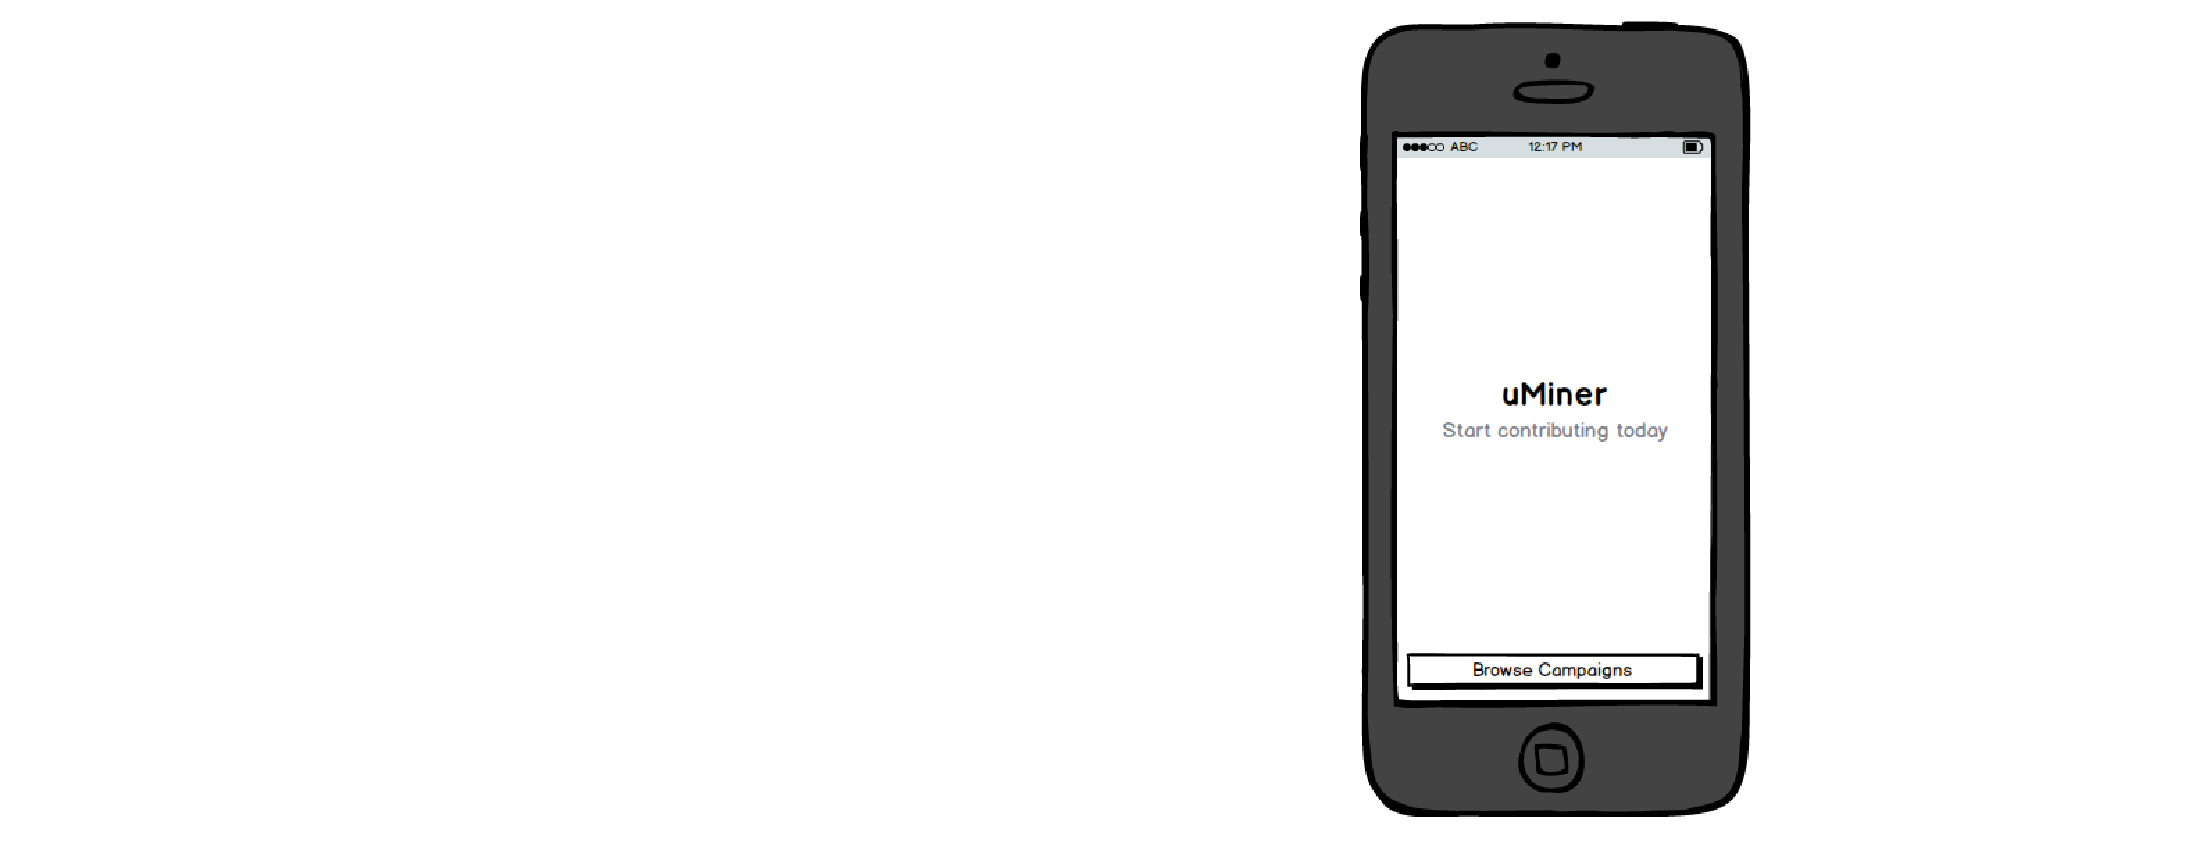
\includegraphics[width=.8\linewidth]{mockups/homepage}
  \caption{Mockup.}
  \label{fig:mockup_initial_screen}
\end{subfigure}%
\begin{subfigure}[!t]{.52\textwidth}
  \centering
  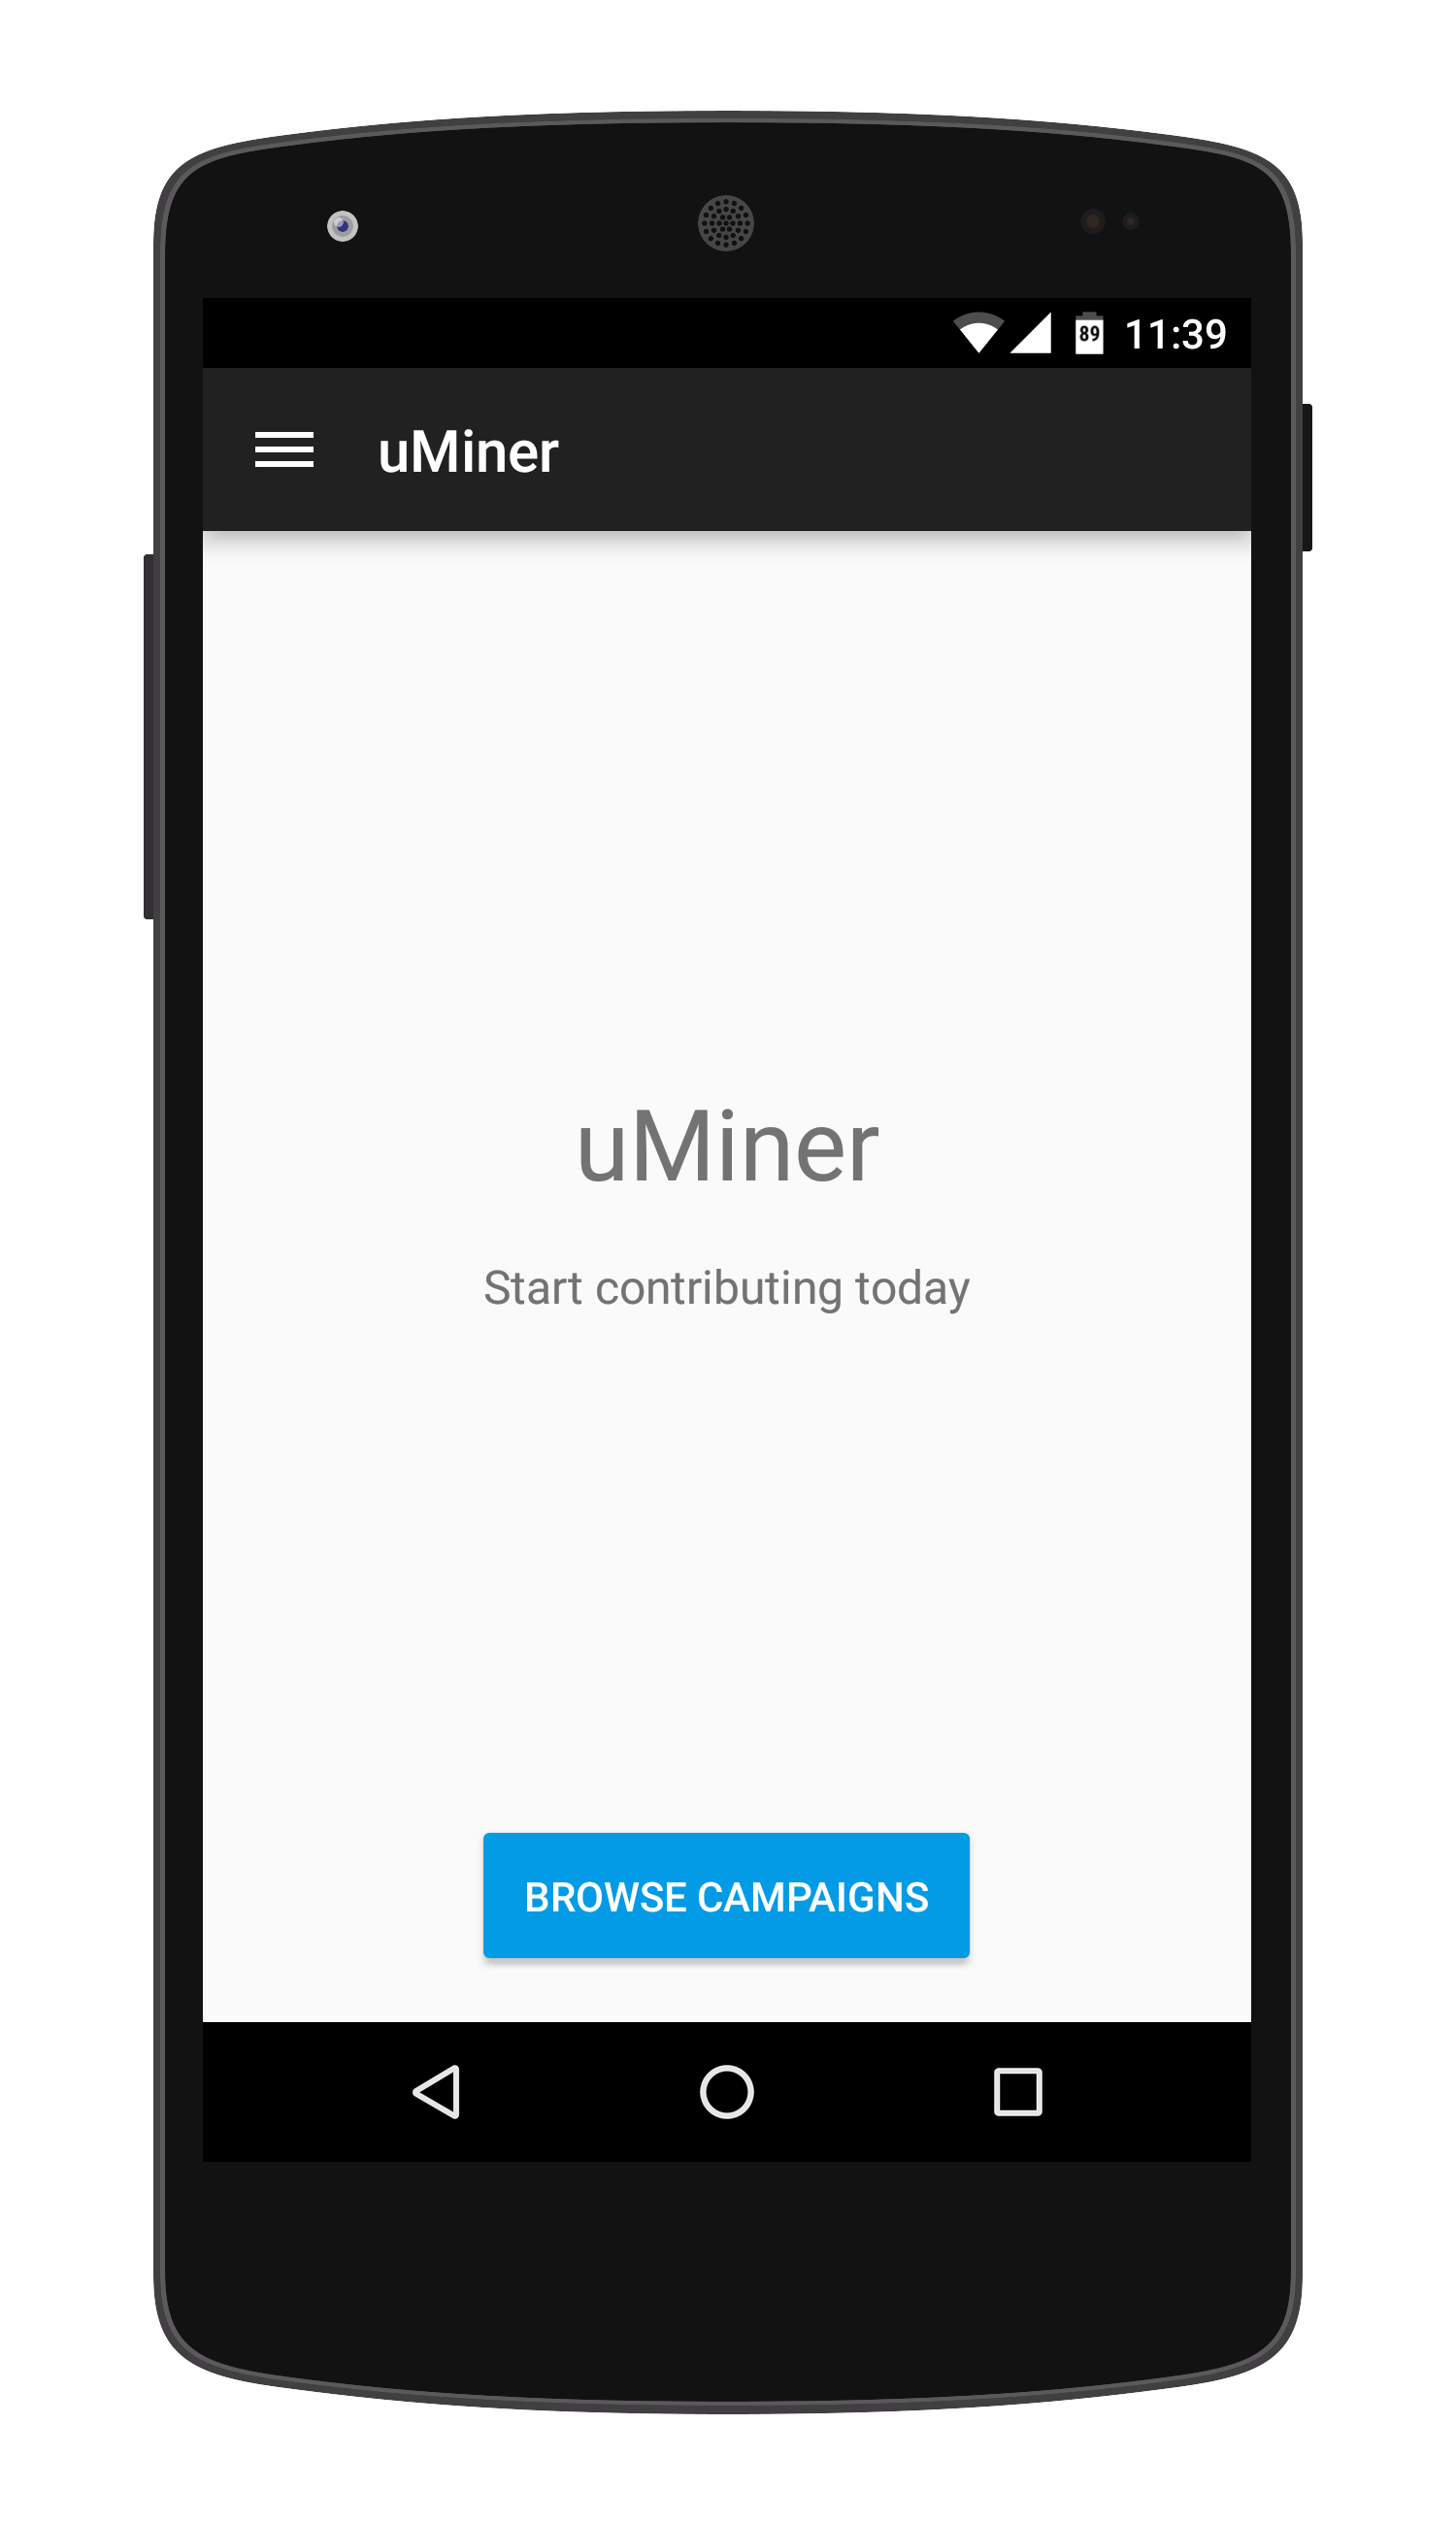
\includegraphics[width=.83\linewidth]{user_interfaces/client_uminer_home_with_phone}
  \caption{Implementation.}
  \label{fig:implementation_initial_screen}
\end{subfigure}
\caption{Initial screen of the Application.}
\label{fig:initial_screen}
\end{figure}
\FloatBarrier

% Navigation
\begin{figure}
\centering
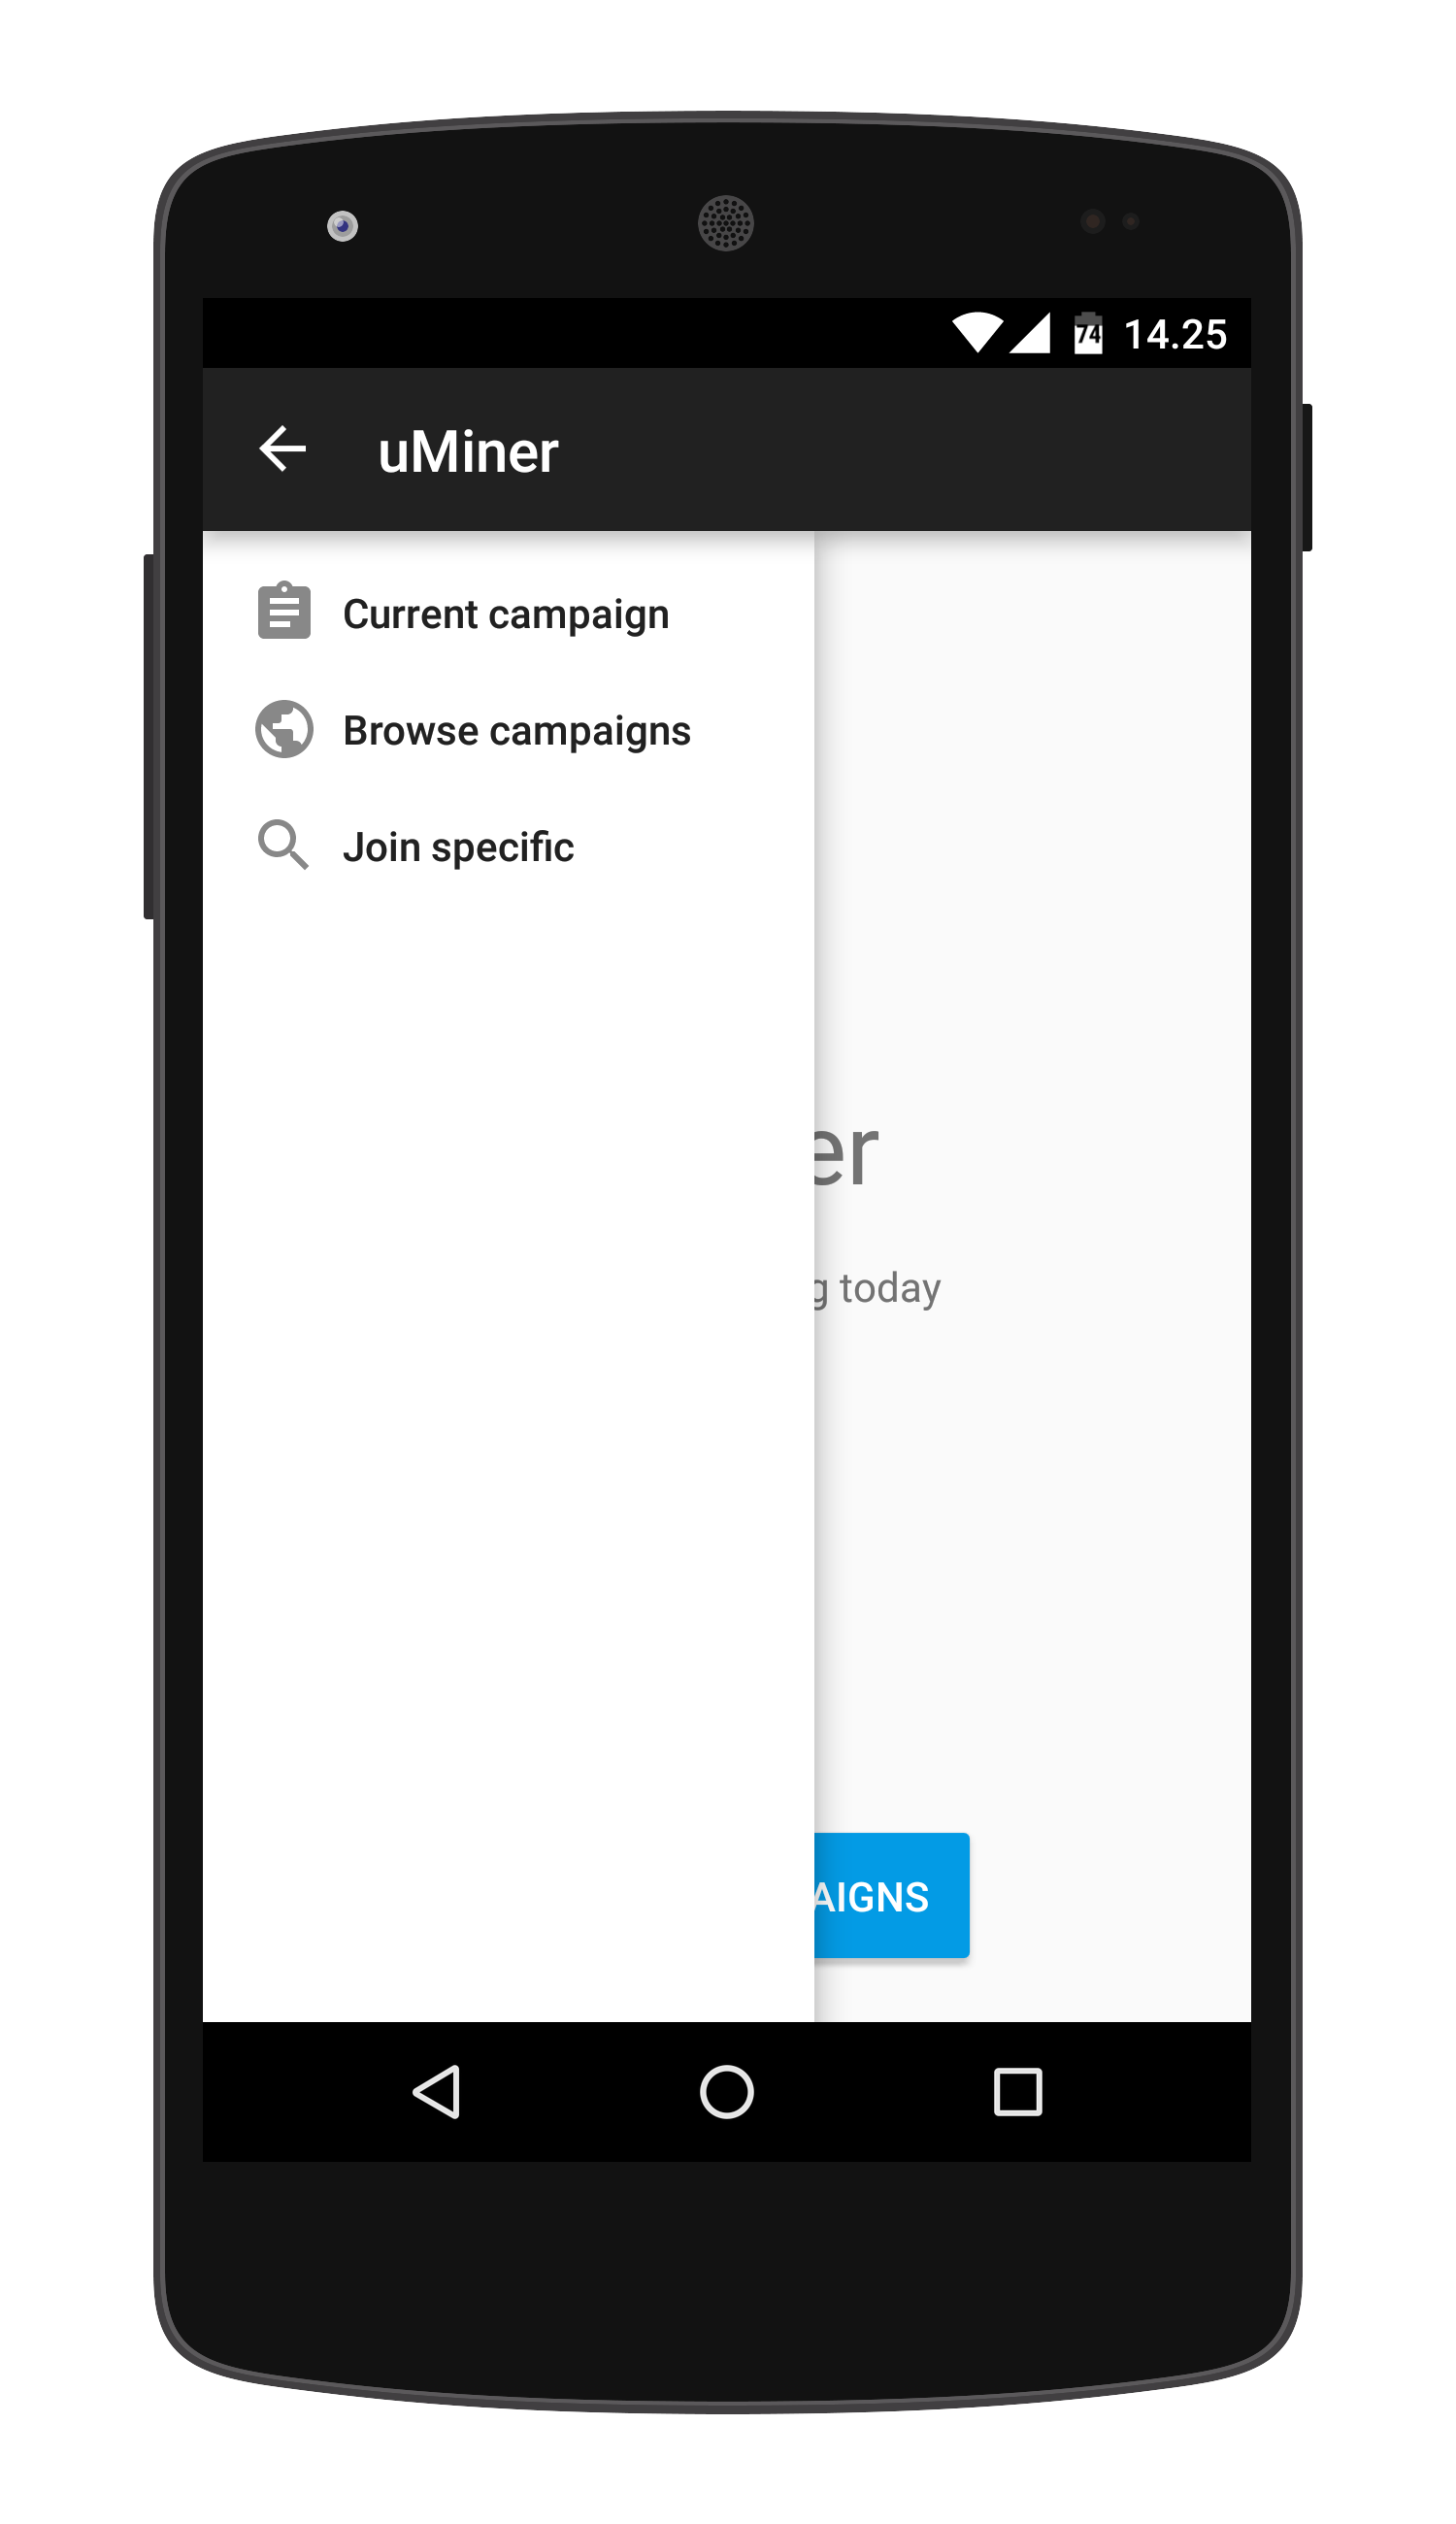
\includegraphics[width=.41\linewidth]{user_interfaces/client_drawer_menu_with_phone}
\caption{Navigation through the application.}
\label{fig:navigation}
\end{figure}
\FloatBarrier

% Publicly available campaigns
\begin{figure}
\begin{subfigure}[!t]{.48\textwidth}
  \centering
  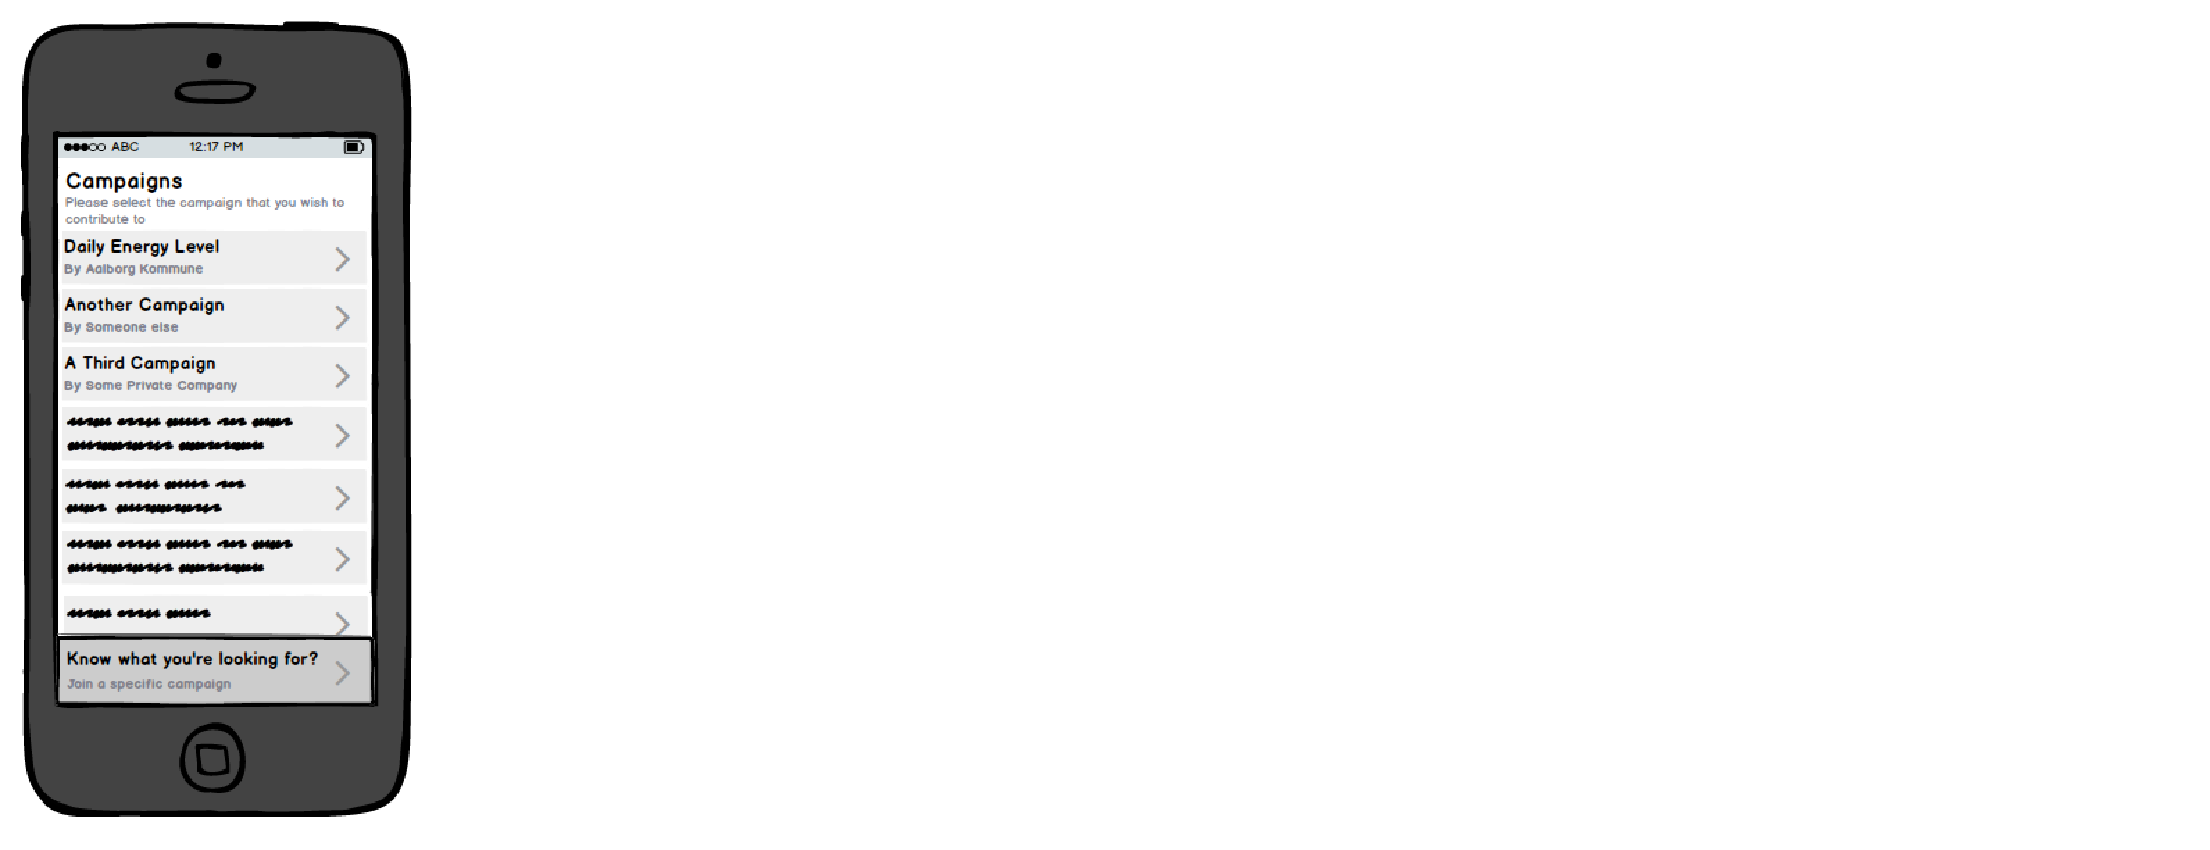
\includegraphics[width=.8\linewidth]{mockups/campaigns_list}
  \caption{Mockup.}
  \label{fig:mockup_public_campaigns}
\end{subfigure}%
\begin{subfigure}[!t]{.52\textwidth}
  \centering
  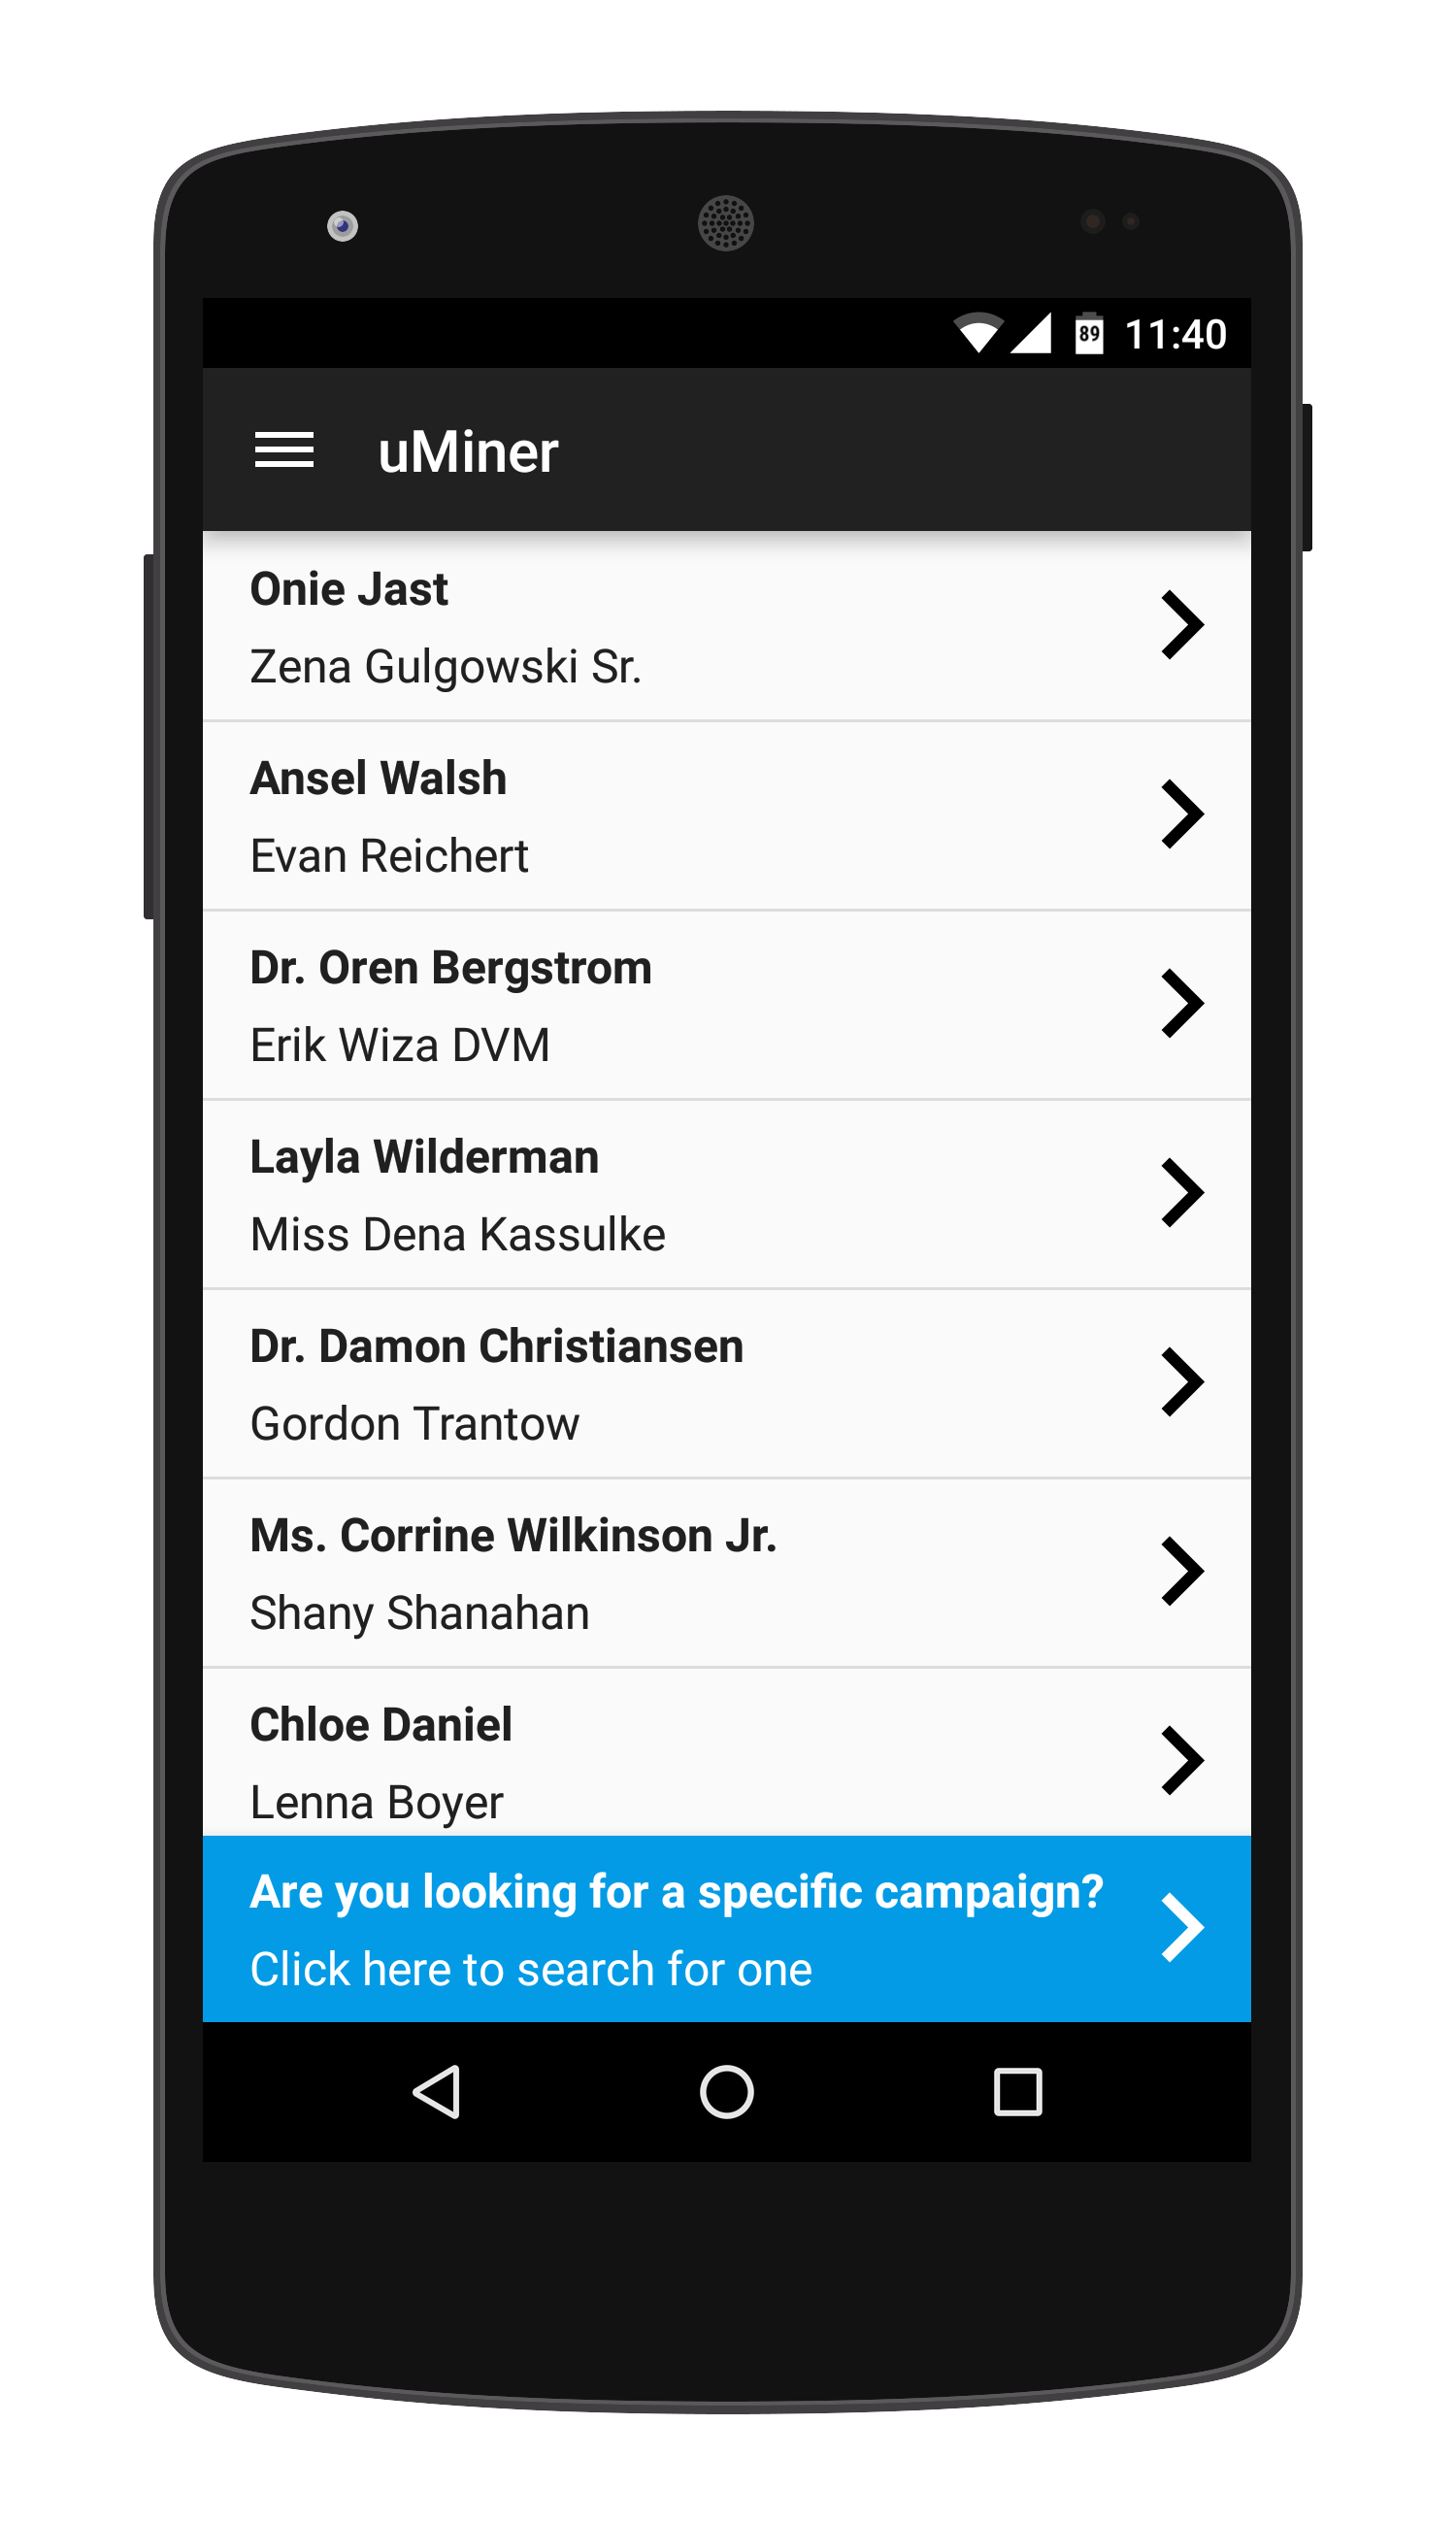
\includegraphics[width=.83\linewidth]{user_interfaces/client_public_campaigns_with_phone}
  \caption{Implementation.}
  \label{fig:implementation_public_campaigns}
\end{subfigure}
\caption{List of publicly available campaigns.}
\label{fig:public_campaigns}
\end{figure}
\FloatBarrier

% Search for a campaign through a campaign identifier
\begin{figure}
\begin{subfigure}[!t]{.48\textwidth}
  \centering
  
\includegraphics[width=.8\linewidth]{mockups/join_specific_campaign}
  \caption{Mockup.}
  \label{fig:mockup_specific_campaign}
\end{subfigure}%
\begin{subfigure}[!t]{.52\textwidth}
  \centering
  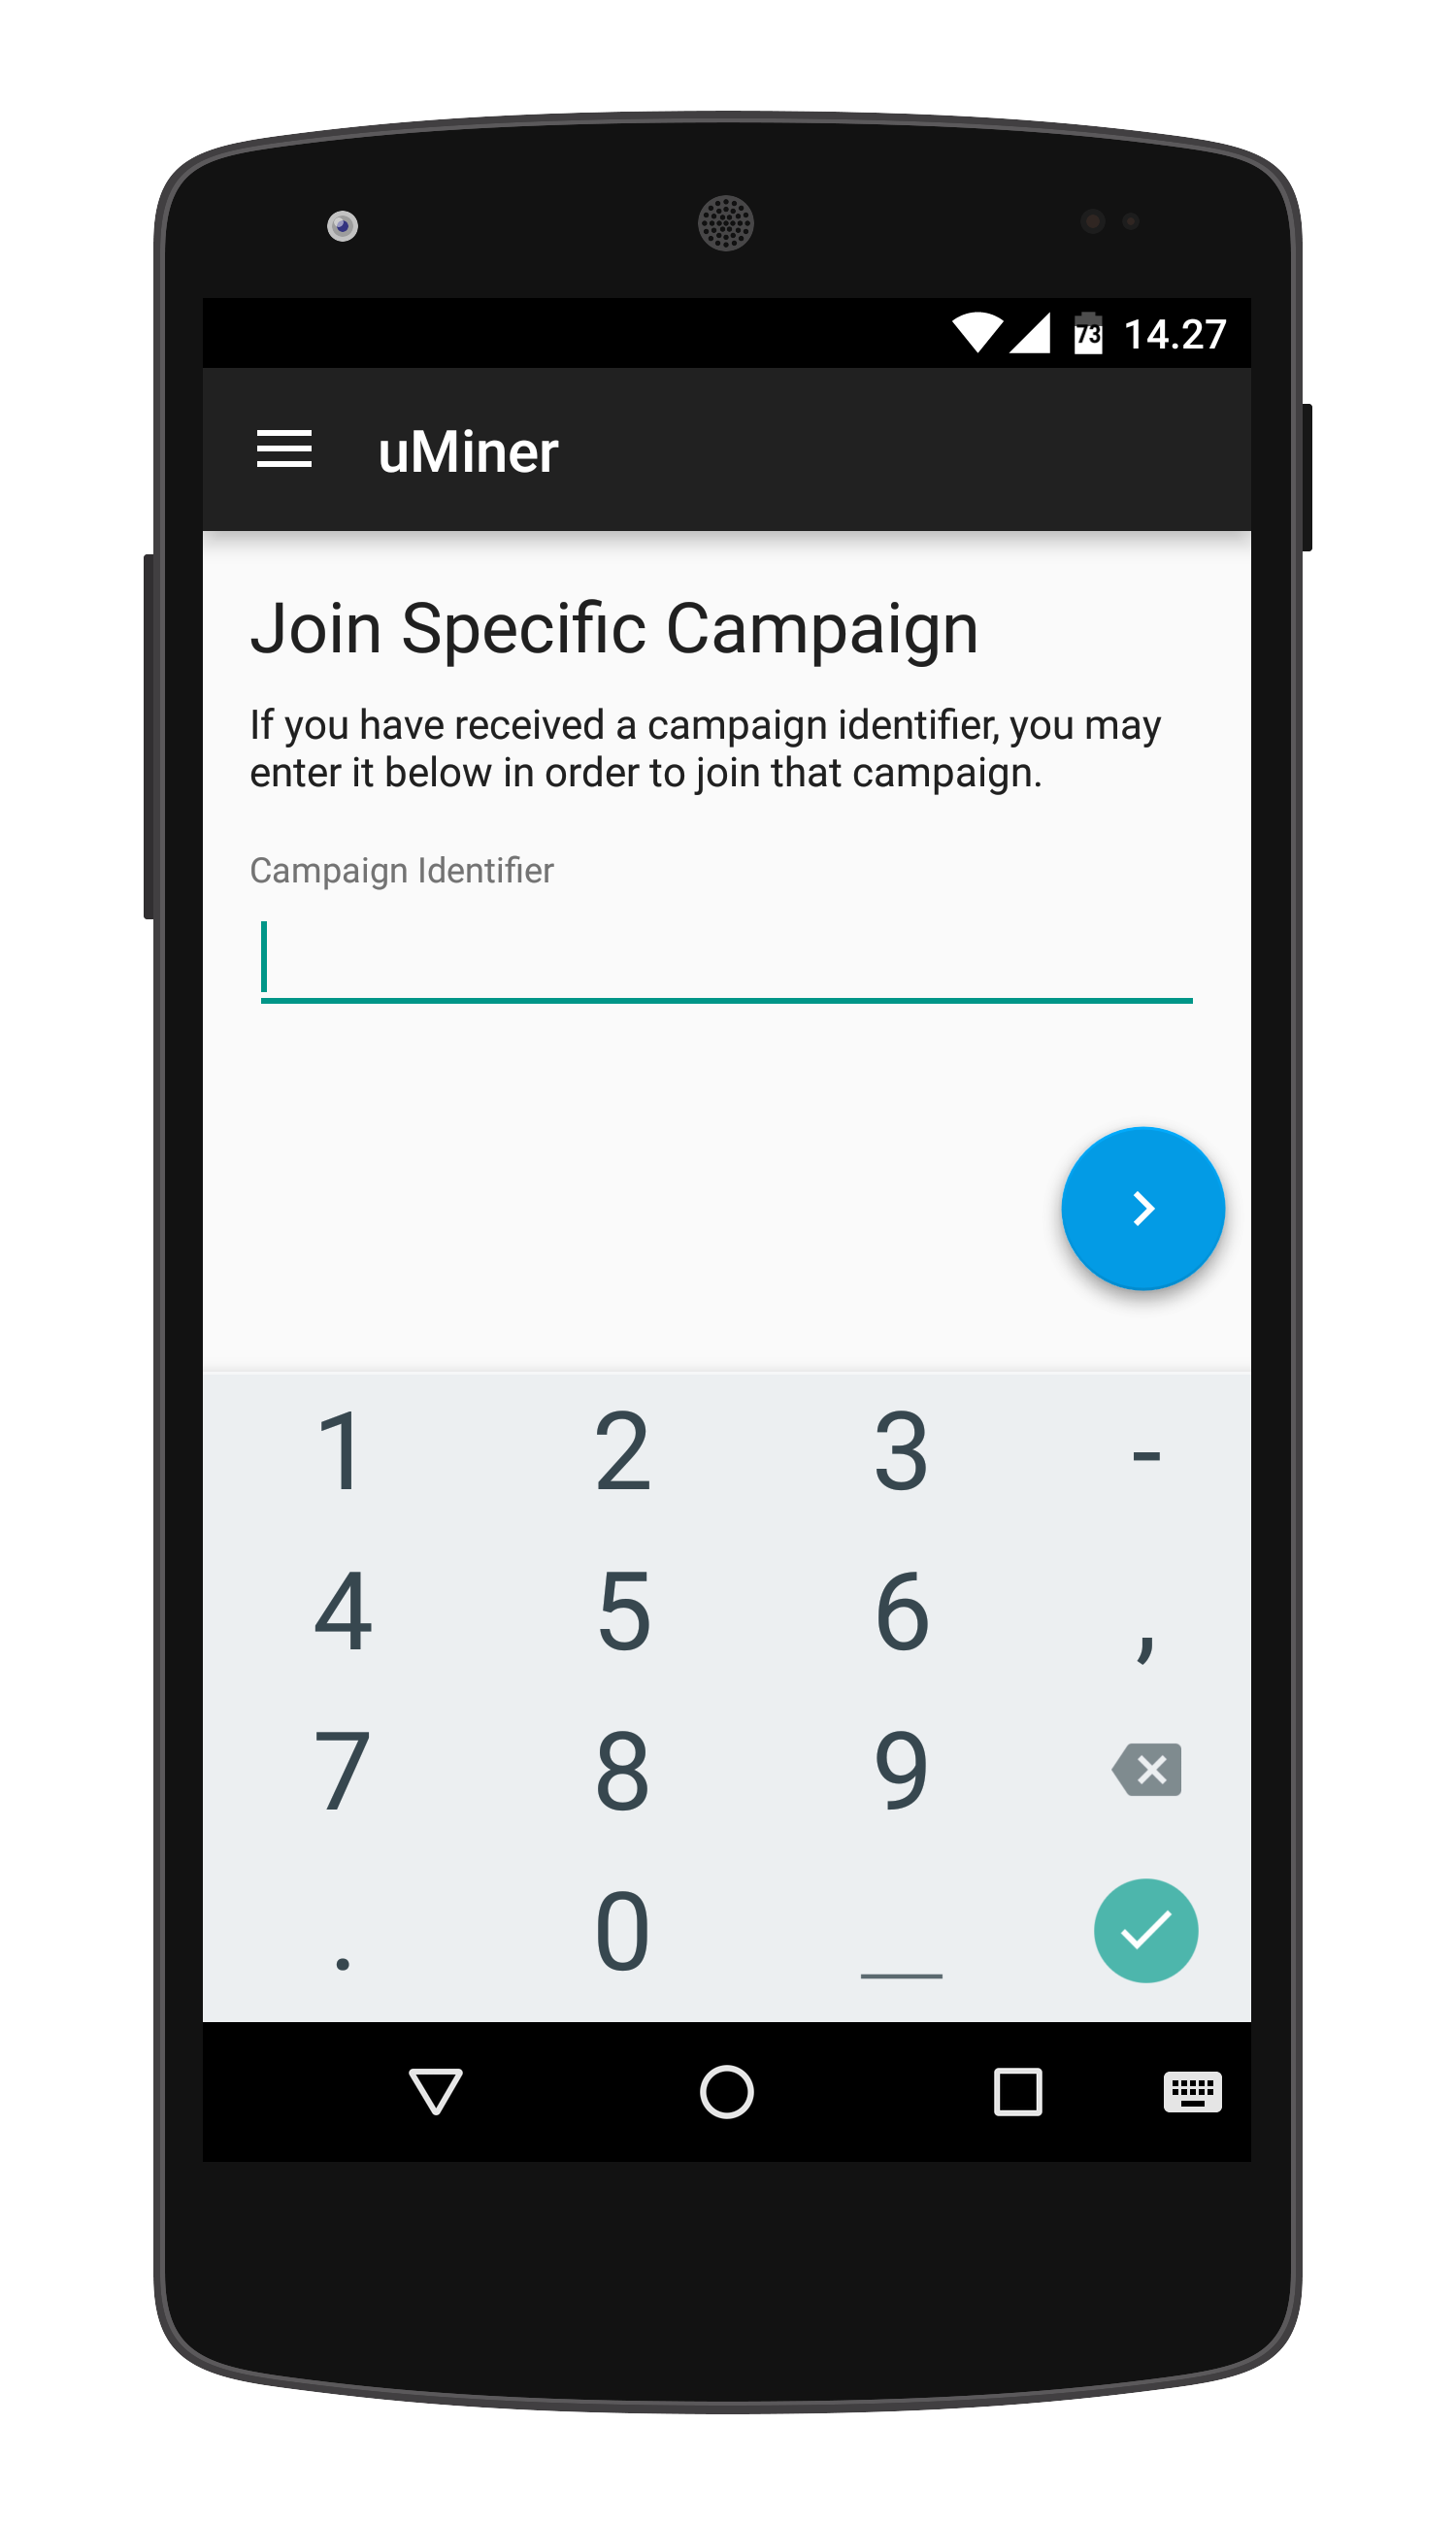
\includegraphics[width=.83\linewidth]{user_interfaces/client_join_specific_campaign_with_phone}
  \caption{Implementation.}
  \label{fig:implementation_specific_campaign}
\end{subfigure}
\caption{Search for a specific campaign using a campaign identifier.}
\label{fig:specific_campaign}
\end{figure}
\FloatBarrier

% Search for a campaign through a campaign identifier
\begin{figure}
\begin{subfigure}[!t]{.48\textwidth}
  \centering
  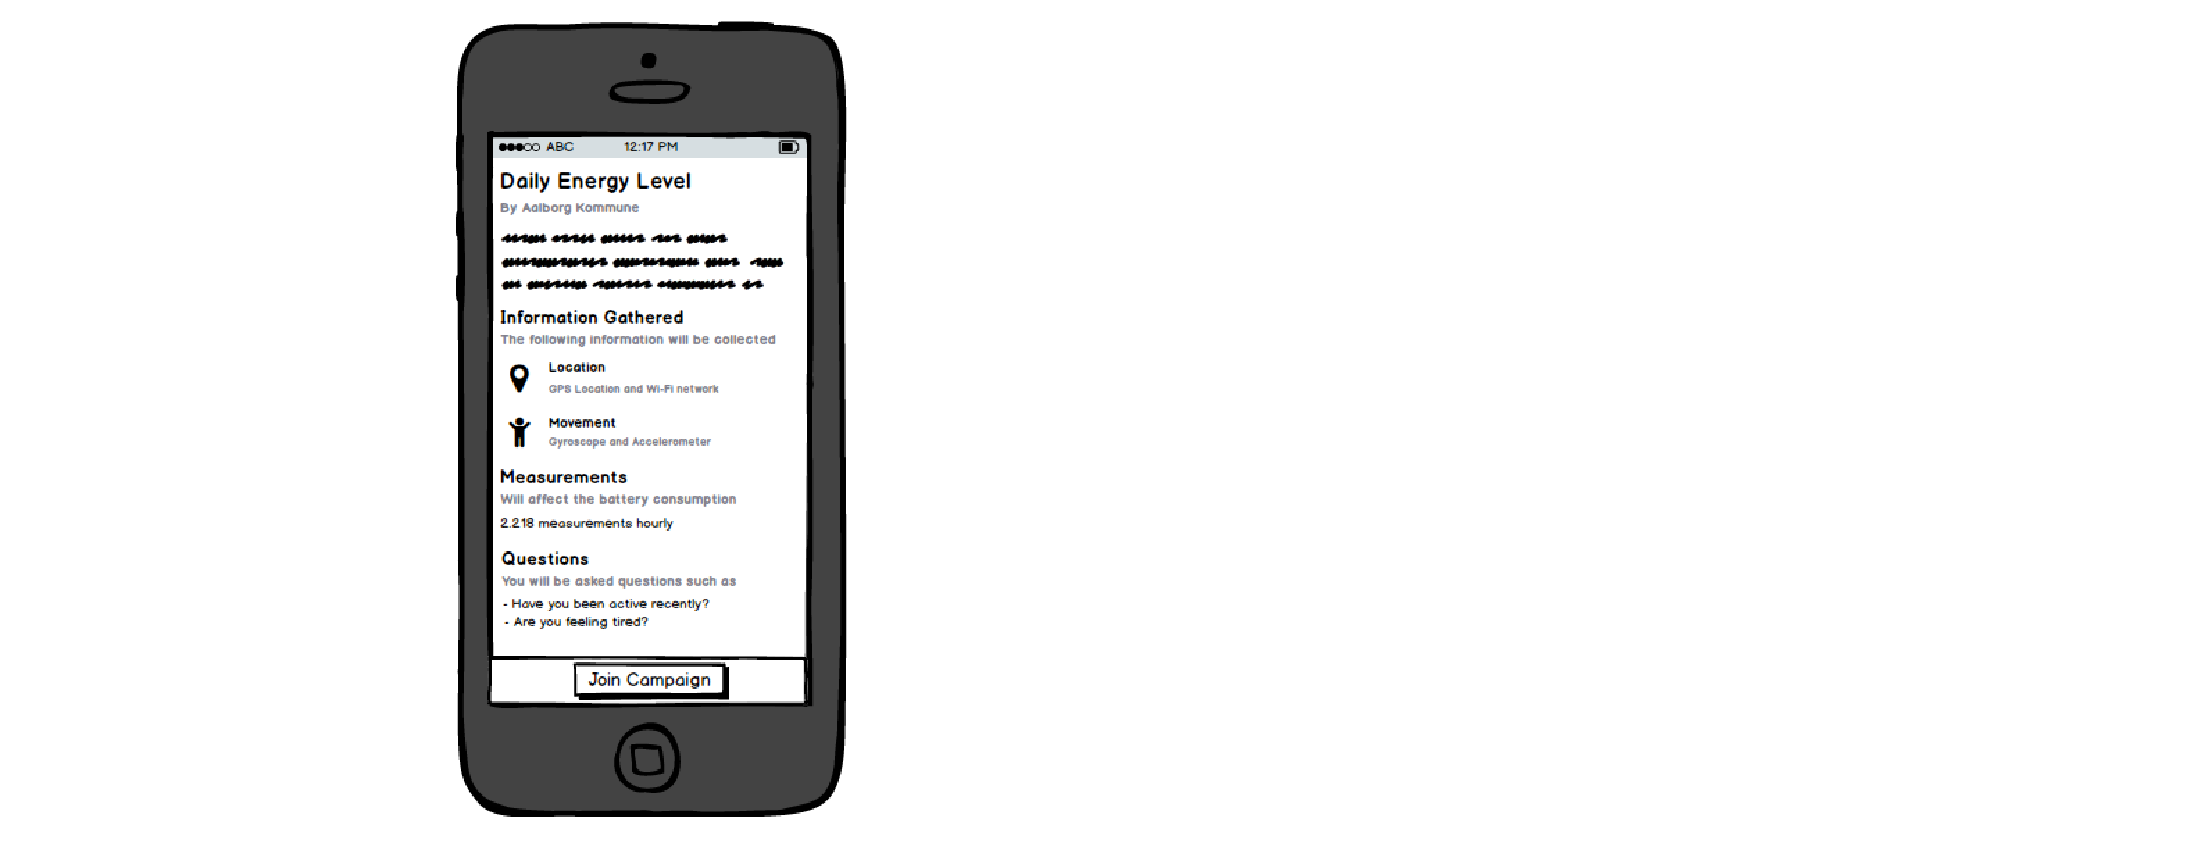
\includegraphics[width=.8\linewidth]{mockups/campaign_specification}
  \caption{Mockup.}
  \label{fig:mockup_campaign_specification}
\end{subfigure}%
\begin{subfigure}[!t]{.52\textwidth}
  \centering
  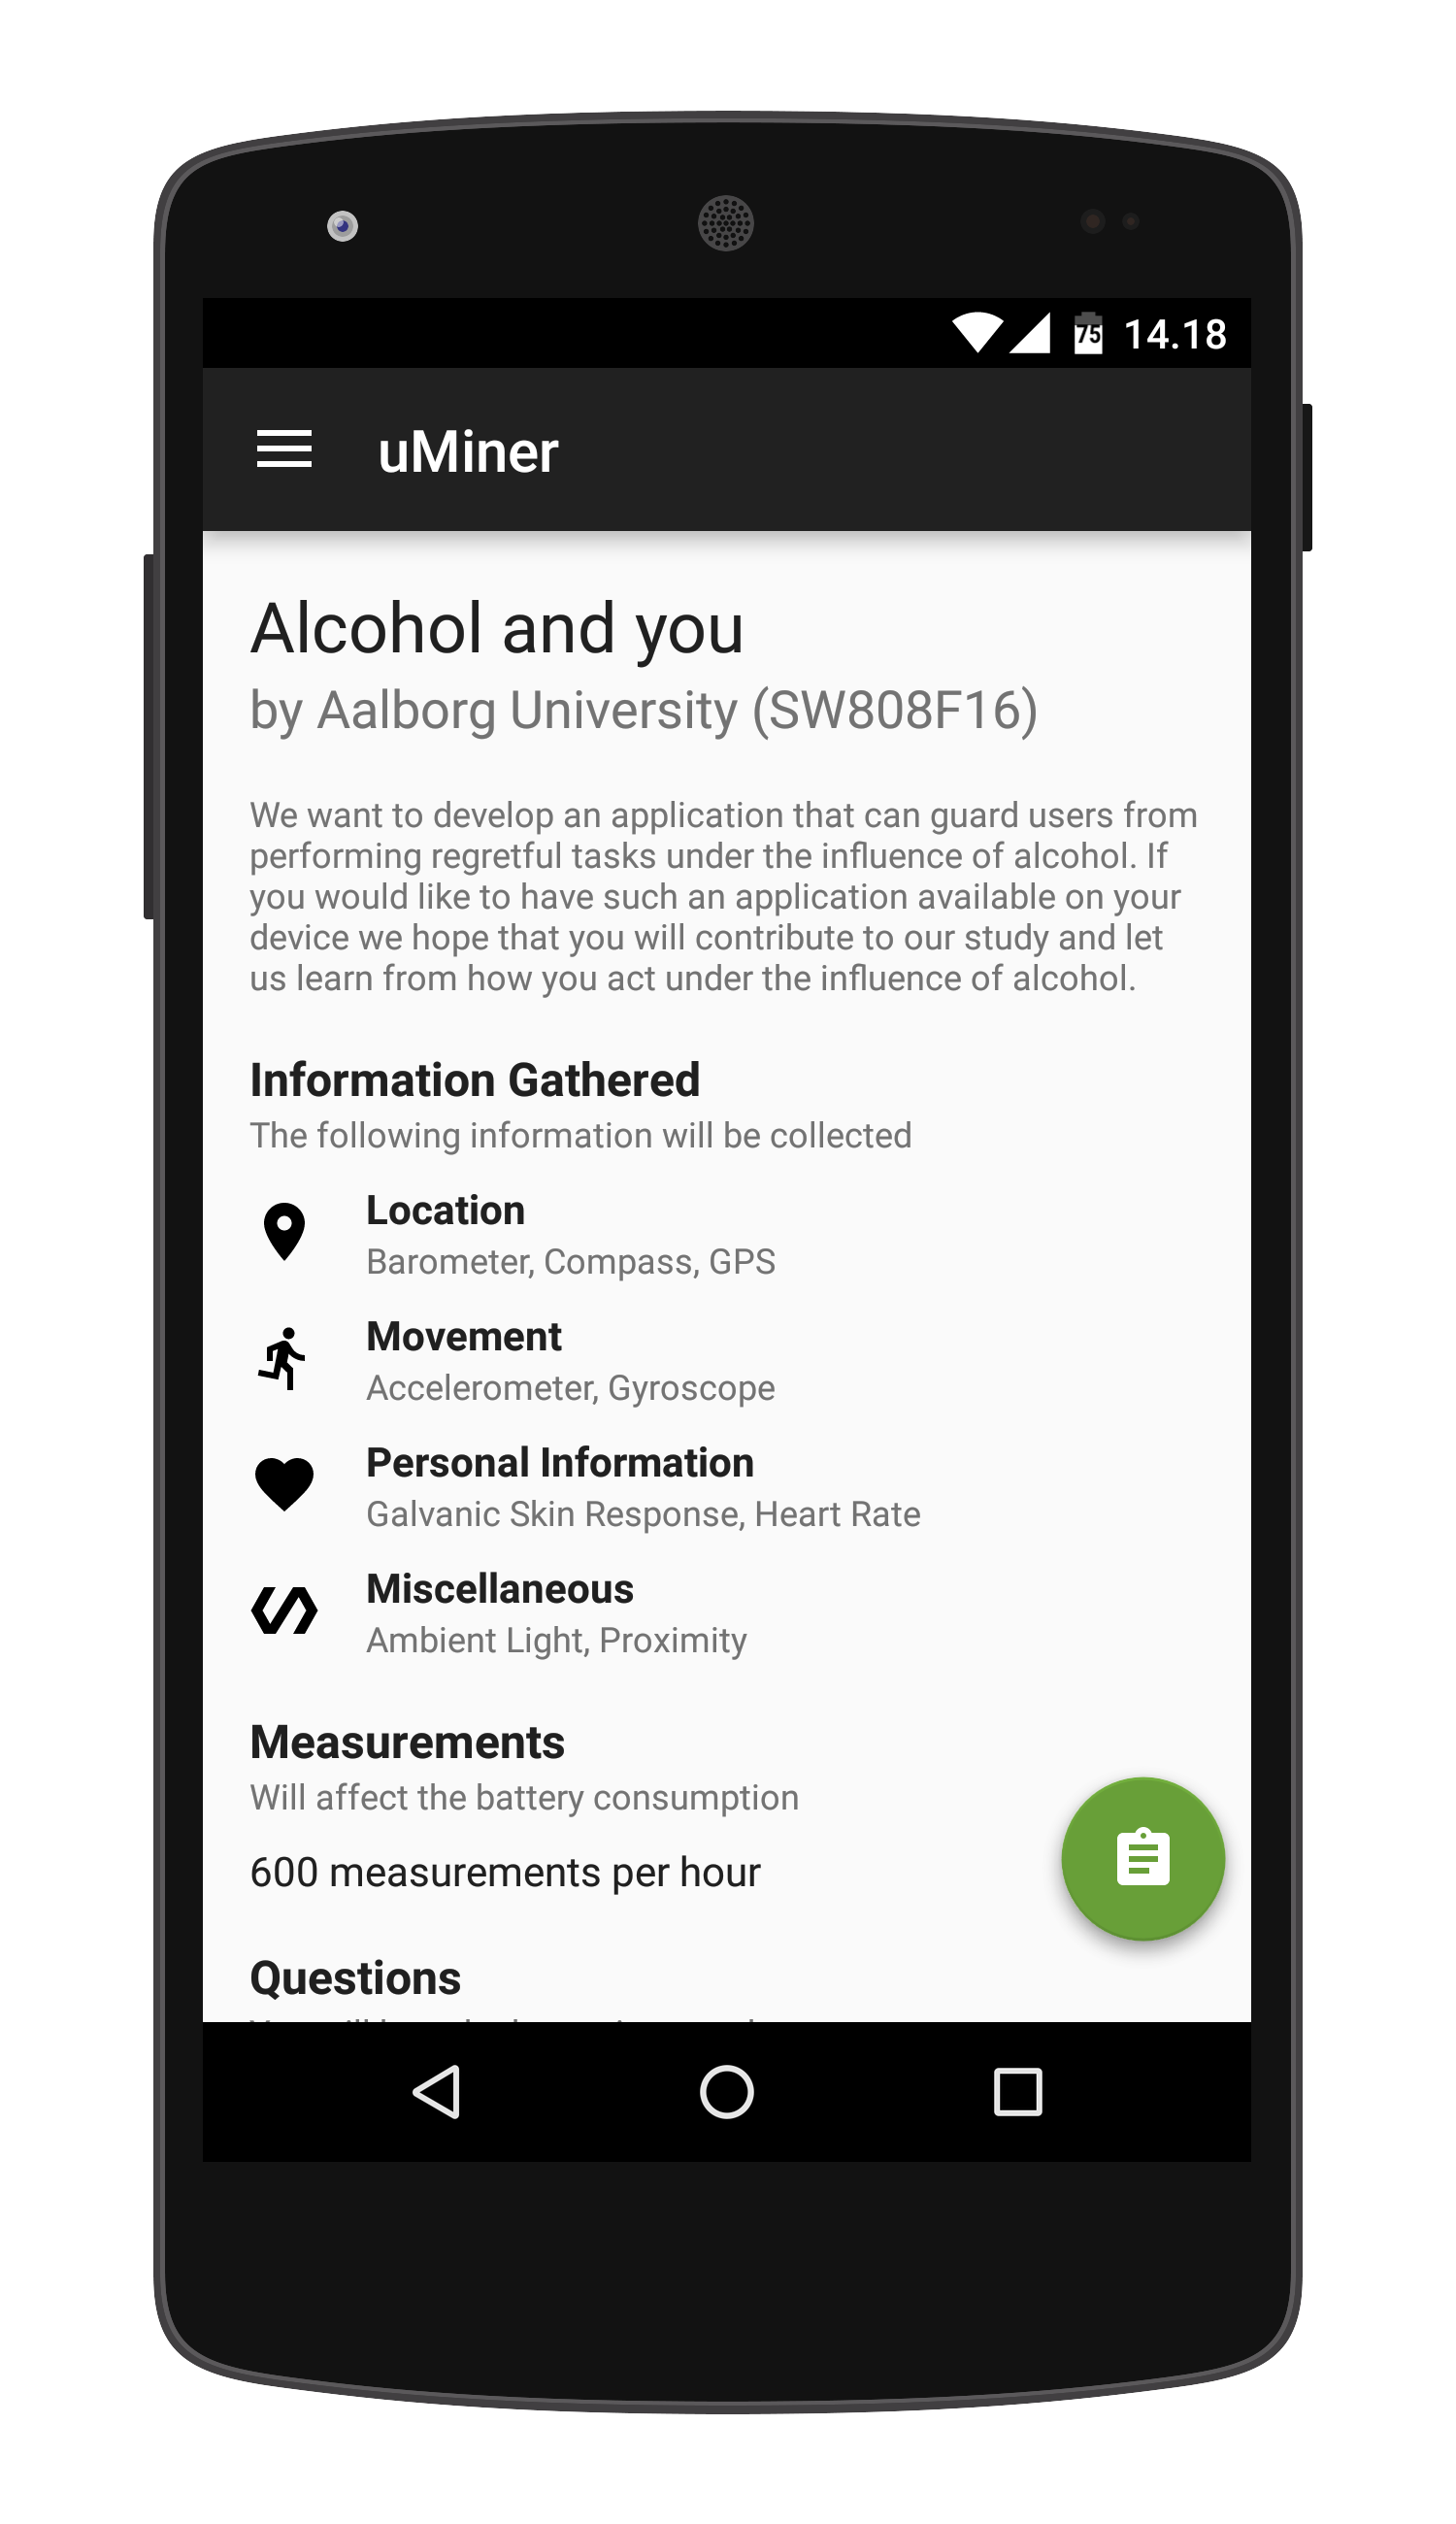
\includegraphics[width=.83\linewidth]{user_interfaces/client_campaign_specification2_with_phone}
  \caption{Implementation.}
  \label{fig:implementation_campaign_specification}
\end{subfigure}
\caption{Campaign specification view.}
\label{fig:campaign_specification}
\end{figure}
\FloatBarrier

% Answering questionnaires
\begin{figure}
\begin{subfigure}[!t]{.50\textwidth}
  \centering
  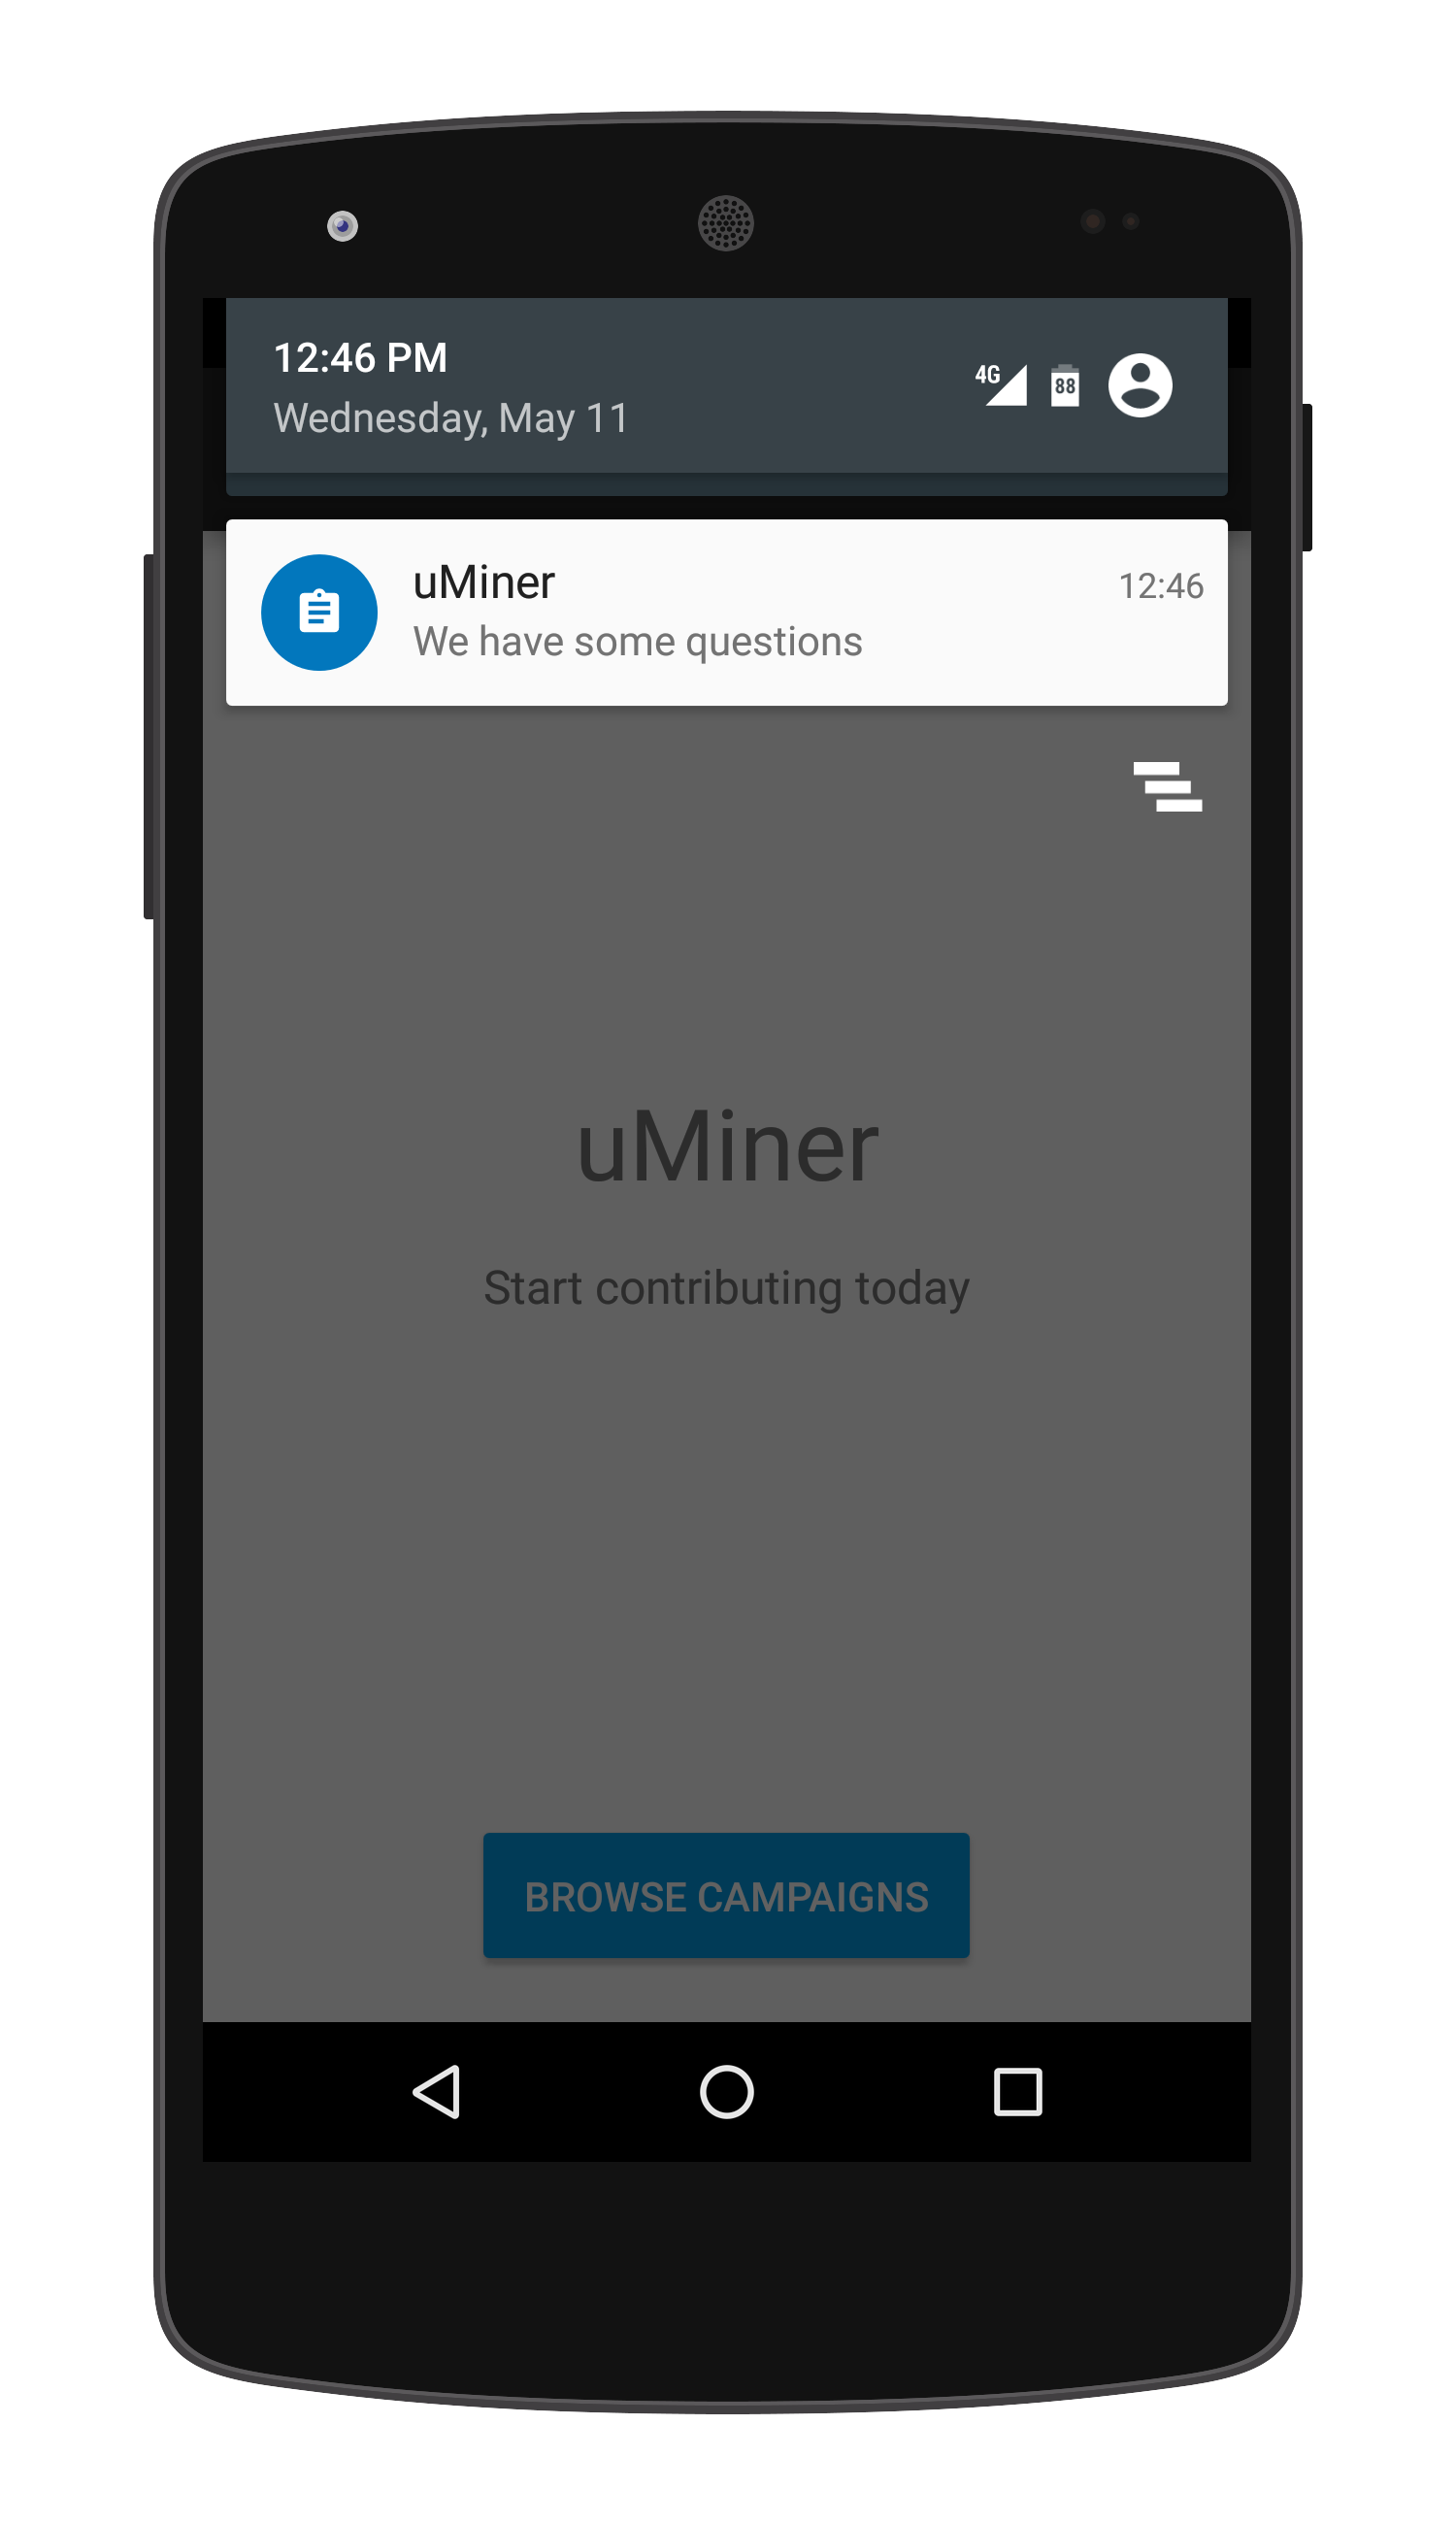
\includegraphics[width=.83\linewidth]{user_interfaces/client_notification_with_phone}
  \caption{Questionnaire notification.}
  \label{fig:answering_questionnaire_notification}
\end{subfigure}%
\begin{subfigure}[!t]{.50\textwidth}
  \centering
  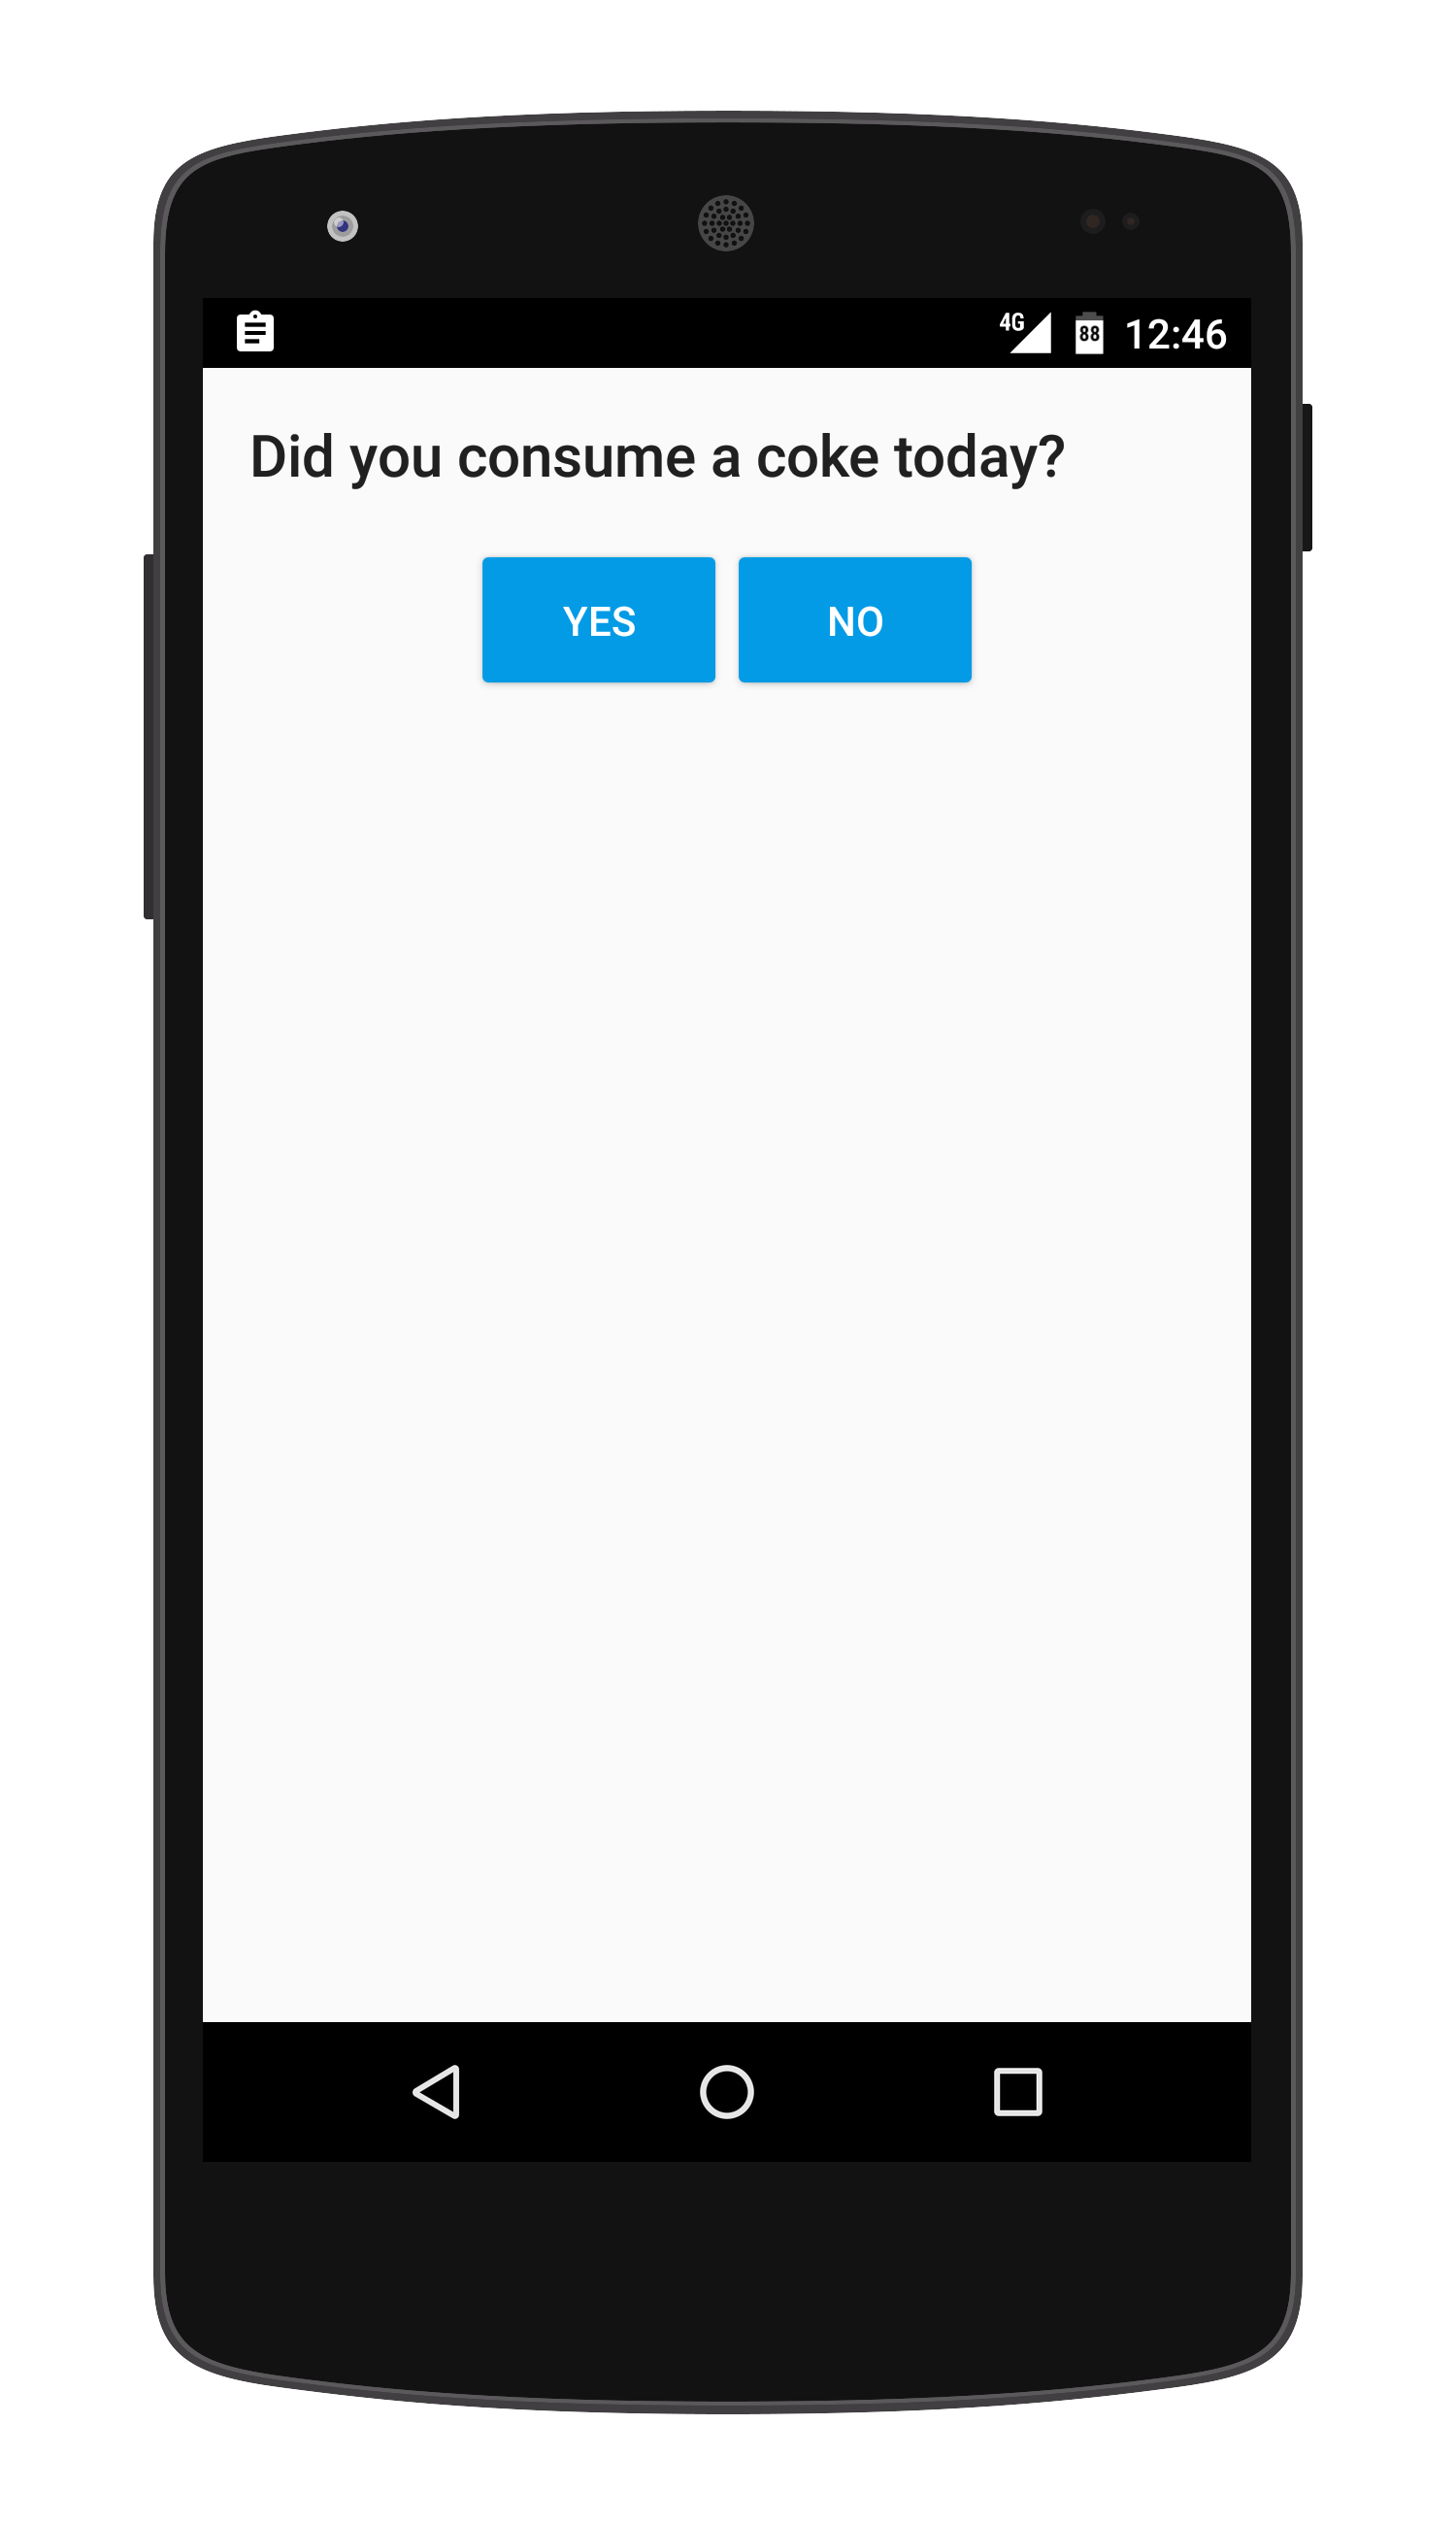
\includegraphics[width=.83\linewidth]{user_interfaces/client_answering_questions_with_phone}
  \caption{Answering the questionnaire.}
  \label{fig:answering_questionnaire_answering}
\end{subfigure}
\caption{Notification regarding questionnaire and answer view.}
\label{fig:answering_questionnaire}
\end{figure}
\FloatBarrier